% ============================================================================
% Campus Biometric Gate Entry Management System — Beamer Presentation
% Main File: Compile this with pdflatex or upload to Overleaf
% ============================================================================
\documentclass[aspectratio=169, 11pt]{beamer}

% ----------------------------------------------------------------------------
% THEME & STYLING (CLEAN, SHADOW-FREE ACADEMIC THEME)
% ----------------------------------------------------------------------------
\usetheme{Madrid}
\usefonttheme{professionalfonts}

% Custom colour palette — deep academic navy + rich gold + modern status tones
\definecolor{PrimaryBlue}{RGB}{16, 37, 78}
\definecolor{SecondaryBlue}{RGB}{28, 62, 126}
\definecolor{AccentGold}{RGB}{205, 155, 30}
\definecolor{LightBg}{RGB}{246, 248, 252}
\definecolor{CodeGreen}{RGB}{28, 138, 56}
\definecolor{DangerRed}{RGB}{198, 40, 40}
\definecolor{InfoBlue}{RGB}{13, 110, 153}
\definecolor{BorderGray}{RGB}{218, 224, 233}

% Beamer Palette Overrides
\setbeamercolor{palette primary}{bg=PrimaryBlue, fg=white}
\setbeamercolor{palette secondary}{bg=SecondaryBlue, fg=white}
\setbeamercolor{palette tertiary}{bg=PrimaryBlue, fg=white}
\setbeamercolor{palette quaternary}{bg=AccentGold, fg=PrimaryBlue}
\setbeamercolor{structure}{fg=PrimaryBlue}
\setbeamercolor{title}{fg=white, bg=PrimaryBlue}
\setbeamercolor{frametitle}{fg=white, bg=PrimaryBlue}

% ----------------------------------------------------------------------------
% CRITICAL FIX: Custom Robust Shadow-Free Block Templates
% Eliminates all black rectangle / drop-shadow shading bugs in Overleaf & PDF viewers
% ----------------------------------------------------------------------------
\setbeamercolor{block title}{bg=PrimaryBlue, fg=white}
\setbeamercolor{block body}{bg=LightBg, fg=black}
\setbeamercolor{block title alerted}{bg=DangerRed, fg=white}
\setbeamercolor{block body alerted}{bg=DangerRed!8, fg=black}
\setbeamercolor{block title example}{bg=CodeGreen, fg=white}
\setbeamercolor{block body example}{bg=CodeGreen!8, fg=black}
\setbeamercolor{item}{fg=PrimaryBlue}

% Use clean standard blocks with NO shading engine
\setbeamertemplate{blocks}[default]

\setbeamertemplate{block begin}{
  \vskip\smallskipamount
  \begin{beamercolorbox}[colsep*=0.75ex,rounded=true]{block title}%
    \usebeamerfont*{block title}\textbf{\insertblocktitle}%
  \end{beamercolorbox}%
  {\parskip0pt\par}%
  \ifbeamercolorempty[bg]{block title}{}{\nointerlineskip\vskip-0.5pt}%
  \usebeamerfont{block body}%
  \begin{beamercolorbox}[colsep*=0.75ex,rounded=true,vmode]{block body}%
    \ifbeamercolorempty[bg]{block body}{\vskip-.25ex}{\vskip-.5ex}\vbox{}%
}
\setbeamertemplate{block end}{
  \end{beamercolorbox}\vskip\smallskipamount
}

\setbeamertemplate{block alerted begin}{
  \vskip\smallskipamount
  \begin{beamercolorbox}[colsep*=0.75ex,rounded=true]{block title alerted}%
    \usebeamerfont*{block title alerted}\textbf{\insertblocktitle}%
  \end{beamercolorbox}%
  {\parskip0pt\par}%
  \ifbeamercolorempty[bg]{block title alerted}{}{\nointerlineskip\vskip-0.5pt}%
  \usebeamerfont{block body alerted}%
  \begin{beamercolorbox}[colsep*=0.75ex,rounded=true,vmode]{block body alerted}%
    \ifbeamercolorempty[bg]{block body alerted}{\vskip-.25ex}{\vskip-.5ex}\vbox{}%
}
\setbeamertemplate{block alerted end}{
  \end{beamercolorbox}\vskip\smallskipamount
}

\setbeamertemplate{block example begin}{
  \vskip\smallskipamount
  \begin{beamercolorbox}[colsep*=0.75ex,rounded=true]{block title example}%
    \usebeamerfont*{block title example}\textbf{\insertblocktitle}%
  \end{beamercolorbox}%
  {\parskip0pt\par}%
  \ifbeamercolorempty[bg]{block title example}{}{\nointerlineskip\vskip-0.5pt}%
  \usebeamerfont{block body example}%
  \begin{beamercolorbox}[colsep*=0.75ex,rounded=true,vmode]{block body example}%
    \ifbeamercolorempty[bg]{block body example}{\vskip-.25ex}{\vskip-.5ex}\vbox{}%
}
\setbeamertemplate{block example end}{
  \end{beamercolorbox}\vskip\smallskipamount
}

% Footer with clean metadata and slide numbers
\setbeamertemplate{navigation symbols}{}
\setbeamertemplate{footline}{
  \leavevmode\hbox{%
    \begin{beamercolorbox}[wd=.333333\paperwidth,ht=2.25ex,dp=1ex,center]{author in head/foot}%
      \usebeamerfont{author in head/foot}\insertshortauthor
    \end{beamercolorbox}%
    \begin{beamercolorbox}[wd=.333333\paperwidth,ht=2.25ex,dp=1ex,center]{title in head/foot}%
      \usebeamerfont{title in head/foot}\insertshorttitle
    \end{beamercolorbox}%
    \begin{beamercolorbox}[wd=.333333\paperwidth,ht=2.25ex,dp=1ex,right]{date in head/foot}%
      \usebeamerfont{date in head/foot}\insertshortdate{}\hspace*{2em}
      \insertframenumber{} / \inserttotalframenumber\hspace*{2ex}
    \end{beamercolorbox}}%
  \vskip0pt%
}

% ----------------------------------------------------------------------------
% PACKAGES
% ----------------------------------------------------------------------------
\usepackage[utf8]{inputenc}
\usepackage[T1]{fontenc}
\usepackage{amsmath, amssymb, amsfonts}
\usepackage{graphicx}
\usepackage{booktabs}
\usepackage{tabularx}
\usepackage{multirow}
\usepackage{listings}
\usepackage{tikz}
\usetikzlibrary{arrows.meta, positioning, shapes.geometric, calc, fit, backgrounds}
\usepackage{xcolor}
\usepackage{hyperref}
\usepackage{fontawesome5}
\usepackage{pifont}

% Code listing style
\lstset{
  basicstyle=\ttfamily\scriptsize,
  keywordstyle=\color{PrimaryBlue}\bfseries,
  commentstyle=\color{gray}\itshape,
  stringstyle=\color{CodeGreen},
  breaklines=true,
  frame=single,
  rulecolor=\color{BorderGray},
  backgroundcolor=\color{LightBg},
  numbers=left,
  numberstyle=\tiny\color{gray},
  tabsize=4,
  showstringspaces=false,
  language=C++
}

% ----------------------------------------------------------------------------
% METADATA
% ----------------------------------------------------------------------------
\title[Campus Biometric Gate System]{
  \textbf{Campus Biometric Gate Entry\\Management System}
}
\subtitle{
  A Dual-Tier C++/Python Architecture with Residency-Aware\\
  State Machine \& ISO/IEC 24745 BioHashing Encryption
}
\author[CS Club Research Team]{
  CS Club Research Team
}
\institute[]{
  Department of Computer Science\\
  \medskip
  \textit{Presented to the Faculty Advisory Committee}
}
\date{August 2026}

% ============================================================================
% BEGIN DOCUMENT
% ============================================================================
\begin{document}

% ---------- SLIDE 1: TITLE SLIDE ----------
\begin{frame}[plain]
  \titlepage
\end{frame}

% ---------- SLIDE 2: TABLE OF CONTENTS ----------
\begin{frame}{Presentation Outline}
  \tableofcontents[hideallsubsections]
\end{frame}

% ============================================================================
\section{Problem Statement \& Motivation}
% ============================================================================

% ---------- SLIDE 3: PROBLEM STATEMENT ----------
\begin{frame}{The Campus Gate Problem}
  \begin{columns}[T]
    \begin{column}{0.55\textwidth}
      \textbf{Critical Pain Points in Current Systems:}
      \begin{itemize}
        \item \textcolor{DangerRed}{\faTimesCircle} \textbf{Manual soft-button selection} — 3--5 sec friction per scan
        \item \textcolor{DangerRed}{\faTimesCircle} \textbf{Touchscreen degradation} — constant physical wear
        \item \textcolor{DangerRed}{\faTimesCircle} \textbf{Buddy punching} — RFID cards are transferable
        \item \textcolor{DangerRed}{\faTimesCircle} \textbf{No leave reconciliation} — false curfew alerts
        \item \textcolor{DangerRed}{\faTimesCircle} \textbf{Plaintext biometric storage} — privacy breach liability
      \end{itemize}
      \vspace{0.3em}
      \begin{alertblock}{Peak Hour Queue Collapse}
        At $\lambda \approx 30$ students/min, standard biometric terminals ($1/\mu \approx 6$ sec) produce $\rho = 3.0$ $\Rightarrow$ \textbf{infinite queue growth}.
      \end{alertblock}
    \end{column}
    \begin{column}{0.42\textwidth}
      \begin{block}{Industry Landscape}
        \small
        \begin{tabular}{ll}
          \toprule
          \textbf{Vendor} & \textbf{Direction Method} \\
          \midrule
          ZKTeco & Manual button \\
          Hikvision & Dual readers \\
          Suprema & Dual readers \\
          HID Mercury & Dual IR sensors \\
          Lenel OnGuard & Dual IR sensors \\
          \midrule
          \textbf{Our System} & \textcolor{CodeGreen}{\textbf{Software only}} \\
          \bottomrule
        \end{tabular}
      \end{block}
    \end{column}
  \end{columns}
\end{frame}

% ============================================================================
\section{System Architecture}
% ============================================================================

% ---------- SLIDE 4: SYSTEM ARCHITECTURE ----------
\begin{frame}{Dual-Tier Decoupled Architecture}
  \begin{center}
  \begin{tikzpicture}[
      scale=0.88, every node/.style={transform shape},
      box/.style={rectangle, draw=PrimaryBlue, fill=PrimaryBlue!8, thick, rounded corners=3pt, minimum width=3.1cm, minimum height=0.72cm, font=\small, align=center},
      bigbox/.style={rectangle, draw=PrimaryBlue, fill=white, thick, rounded corners=4pt, minimum width=13.0cm, minimum height=0.9cm, font=\small\bfseries, align=center},
      arrow/.style={-{Stealth[length=2.5mm]}, thick, PrimaryBlue}
    ]

    % Python Layer
    \node[bigbox, fill=AccentGold!15] (python) at (0, 2.6) {\faIcon{python} \textbf{Python Administrative Application Layer} — GUI Panels, Leave Workflows, Excel Reports};

    % Bridge
    \node[rectangle, draw=AccentGold, fill=AccentGold!35, thick, rounded corners=2pt, minimum width=3.2cm, minimum height=0.45cm, font=\scriptsize\bfseries] (bridge) at (0, 1.6) {C-ABI Bridge (\texttt{ctypes})};

    % Engine
    \node[bigbox, fill=PrimaryBlue!10] (engine) at (0, 0.7) {\faIcon{cogs} \textbf{Bare-Metal C++17 Biometric Engine v2.0}};

    % Engine sub-modules (4 boxes evenly spaced across width)
    \node[box] (master)  at (-4.65, -0.45) {Master DB\\(\texttt{master\_db.cpp})};
    \node[box] (indexer) at (-1.55, -0.45) {FNV-1a Indexer\\(\texttt{indexer.cpp})};
    \node[box] (crypto)  at (1.55, -0.45)  {\textcolor{DangerRed}{\faLock} BioHash Crypto\\(\texttt{crypto\_placeholder.cpp})};
    \node[box] (finger)  at (4.65, -0.45)  {Match Delegate\\(\texttt{fingerprint.cpp})};

    % Storage
    \node[bigbox, fill=LightBg, draw=BorderGray] (storage) at (0, -1.6) {\faIcon{database} \textbf{Localized Binary File Store} — \texttt{Student\_data/}, \texttt{Everyday\_data/}, \texttt{biohash.key}};

    % Arrows
    \draw[arrow] (python) -- (bridge);
    \draw[arrow] (bridge) -- (engine);
    \draw[arrow] (engine.south -| master.north) -- (master.north);
    \draw[arrow] (engine.south -| indexer.north) -- (indexer.north);
    \draw[arrow] (engine.south -| crypto.north) -- (crypto.north);
    \draw[arrow] (engine.south -| finger.north) -- (finger.north);
    \draw[arrow] (master.south) -- (master.south |- storage.north);
    \draw[arrow] (indexer.south) -- (indexer.south |- storage.north);
    \draw[arrow, DangerRed] (crypto.east) -- (finger.west);

  \end{tikzpicture}
  \end{center}
\end{frame}

% ============================================================================
\section{Innovation 1: Residency-Aware Parity State Machine}
% ============================================================================

% ---------- SLIDE 5: PARITY STATE MACHINE ----------
\begin{frame}{Zero-Friction Direction Detection}
  \begin{columns}[T]
    \begin{column}{0.48\textwidth}
      \begin{block}{Formal State Transition Rules}
        \small
        Given scan count $n \in \mathbb{N}$ for a student on current date:
        \vspace{0.2em}

        \textbf{Hosteller} (initial state: INSIDE):
        \[
          \text{Status}(n) = \begin{cases}
            \text{OUT} & n \bmod 2 \neq 0 \\
            \text{IN}  & n \bmod 2 = 0
          \end{cases}
        \]

        \textbf{Day Scholar} (initial state: OUTSIDE):
        \[
          \text{Status}(n) = \begin{cases}
            \text{IN}  & n \bmod 2 \neq 0 \\
            \text{OUT} & n \bmod 2 = 0
          \end{cases}
        \]
      \end{block}
    \end{column}
    \begin{column}{0.48\textwidth}
      \begin{exampleblock}{Implementation (C++17)}
        \lstinputlisting[language=C++, firstline=1, lastline=8]{snippets/parity_logic.cpp}
      \end{exampleblock}
      \vspace{0.2em}
      \begin{block}{Key Differentiator}
        \small
        \textbf{Anti-passback:} Dual IR beam-break \textit{hardware}.\\[0.15em]
        \textbf{Our approach:} Software logic + domain metadata.\\[0.15em]
        \textcolor{CodeGreen}{\faCheckCircle} \textbf{Zero additional hardware.}\\
        \textcolor{CodeGreen}{\faCheckCircle} \textbf{Zero manual user input.}
      \end{block}
    \end{column}
  \end{columns}
\end{frame}

% ============================================================================
\section{Innovation 2: BioHashing Cancelable Encryption}
% ============================================================================

% ---------- SLIDE 6: BIOHASHING THEORY (COMPACT MATH — NO OVERFLOW) ----------
\begin{frame}{BioHashing: Random Orthogonal Projection + Binarization}
  \begin{columns}[T]
    \begin{column}{0.53\textwidth}
      \begin{block}{Mathematical Foundation}
        \small
        Raw template $X \in \mathbb{R}^{512}$, key seed $K$, random projection matrix $R \in \mathbb{R}^{512 \times 512}$ generated from $K$:
        \vspace{0.3em}

        \textbf{1. Projection (Dot Product):}
        \[ P_i = \sum_{j=1}^{512} R_{ij} \cdot X_j = R_i \cdot X \]

        \textbf{2. Binarization (Sign Function):}
        \[ Y_i = \begin{cases} 1 & \text{if } P_i \geq 0 \\ 0 & \text{if } P_i < 0 \end{cases} \quad \implies Y \in \{0,1\}^{512} \]

        \textbf{3. Transformed Matching (Hamming):}
        \[ \text{Score} = 1.0 - \frac{d_H(Y_{\text{live}}, Y_{\text{stored}})}{512} \geq 0.75 \]
      \end{block}
    \end{column}
    \begin{column}{0.44\textwidth}
      \begin{block}{ISO/IEC 24745 Compliance}
        \small
        \begin{tabular}{lc}
          \toprule
          \textbf{Property} & \textbf{Status} \\
          \midrule
          Irreversibility & \textcolor{CodeGreen}{\faCheckCircle\ Satisfied} \\
          Unlinkability & \textcolor{CodeGreen}{\faCheckCircle\ Satisfied} \\
          Renewability & \textcolor{CodeGreen}{\faCheckCircle\ Satisfied} \\
          \bottomrule
        \end{tabular}
      \end{block}
      \vspace{0.2em}
      \begin{alertblock}{Security Bounds}
        \small
        \textbf{Key space:} $2^{64} \approx 1.84 \times 10^{19}$\\
        \textbf{Template inversion:} $O(2^{512})$\\
        \textbf{Random collision:} $\approx 10^{-154}$
      \end{alertblock}
    \end{column}
  \end{columns}
\end{frame}

% ---------- SLIDE 7: BUFFER LAYOUT & ENROLLMENT (PERFECTLY CENTERED — NO CLIPPING) ----------
\begin{frame}{Encrypted Template Buffer Layout}
  \begin{center}
  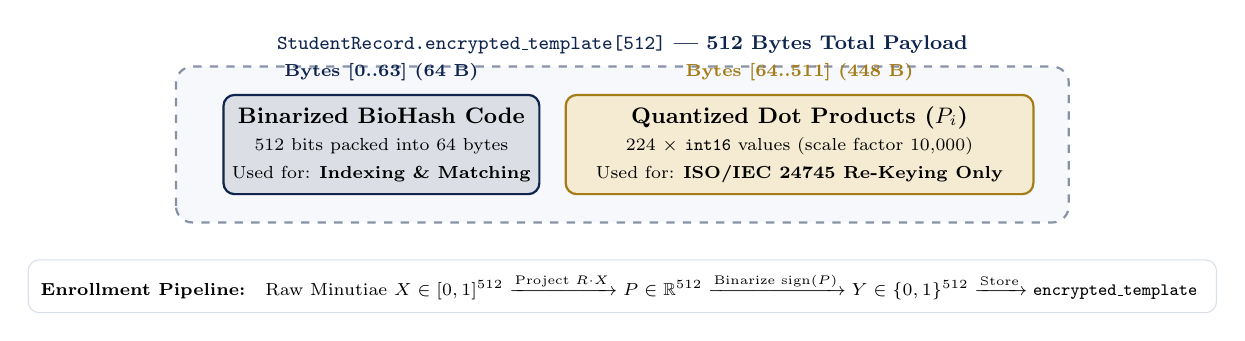
\begin{tikzpicture}[
      scale=0.90, every node/.style={transform shape},
      box/.style={rectangle, draw=PrimaryBlue, thick, rounded corners=4pt, align=center, font=\small},
    ]
    % Surrounding dashed box for total 512 bytes
    \draw[PrimaryBlue!50, dashed, thick, fill=LightBg, rounded corners=6pt] (-6.3, -0.9) rectangle (6.3, 1.3);
    \node[above, font=\footnotesize\bfseries, text=PrimaryBlue] at (0, 1.35) {\texttt{StudentRecord.encrypted\_template[512]} — 512 Bytes Total Payload};

    % Left Box: Binarized BioHash Code (Bytes 0..63)
    \node[box, fill=PrimaryBlue!15, minimum width=4.4cm, minimum height=1.4cm] (bio) at (-3.4, 0.2) {
      \textbf{Binarized BioHash Code}\\
      \scriptsize 512 bits packed into 64 bytes\\
      \scriptsize Used for: \textbf{Indexing \& Matching}
    };
    \node[above=0.06cm of bio, font=\scriptsize\bfseries, text=PrimaryBlue] {Bytes [0..63] (64 B)};

    % Right Box: Quantized Dot Products (Bytes 64..511)
    \node[box, fill=AccentGold!20, draw=AccentGold!80!black, minimum width=6.6cm, minimum height=1.4cm] (dot) at (2.5, 0.2) {
      \textbf{Quantized Dot Products ($P_i$)}\\
      \scriptsize 224 $\times$ \texttt{int16} values (scale factor 10,000)\\
      \scriptsize Used for: \textbf{ISO/IEC 24745 Re-Keying Only}
    };
    \node[above=0.06cm of dot, font=\scriptsize\bfseries, text=AccentGold!80!black] {Bytes [64..511] (448 B)};

    % Pipeline description box below
    \node[rectangle, draw=BorderGray, fill=white, rounded corners=4pt, minimum width=12.6cm, inner sep=5pt, font=\scriptsize, align=center] at (0, -1.8) {
      \textbf{Enrollment Pipeline:}\quad
      $\text{Raw Minutiae } X \in [0,1]^{512}
      \xrightarrow{\text{Project } R \cdot X} P \in \mathbb{R}^{512}
      \xrightarrow{\text{Binarize } \text{sign}(P)} Y \in \{0,1\}^{512}
      \xrightarrow{\text{Store}} \texttt{encrypted\_template}$
    };
  \end{tikzpicture}
  \end{center}
\end{frame}

% ============================================================================
\section{Innovation 3: Dual-Tier Coarse-to-Fine Matching}
% ============================================================================

% ---------- SLIDE 8: DUAL-TIER MATCHING PIPELINE (PERFECT SPACING & CLEAN ARROWS) ----------
\begin{frame}{Dual-Tier Matching Pipeline}
  \begin{center}
  \begin{tikzpicture}[
      scale=0.82, every node/.style={transform shape},
      step/.style={rectangle, draw=PrimaryBlue, fill=PrimaryBlue!8, thick, rounded corners=3pt, minimum width=9.2cm, minimum height=0.55cm, font=\footnotesize, align=center},
      decision/.style={diamond, draw=AccentGold, fill=AccentGold!20, thick, aspect=2.6, font=\scriptsize\bfseries, inner sep=1.2pt},
      branch/.style={rectangle, draw=BorderGray, thick, rounded corners=3pt, minimum width=4.0cm, minimum height=0.5cm, font=\scriptsize, align=center},
      arrow/.style={-{Stealth[length=2mm]}, thick, PrimaryBlue},
    ]

    \node[step] (scan) at (0, 3.6) {\faIcon{fingerprint} \textbf{Live Optical Scan} — 512-byte Raw Template $X_{\text{live}}$};
    \node[step, fill=DangerRed!8] (transform) at (0, 2.7) {\faLock\ \textbf{BioHash Transform} — $Y_{\text{live}} = \text{sign}(R \cdot X_{\text{live}})$ (\texttt{crypto\_enroll\_transform})};
    \node[step] (hash) at (0, 1.8) {\textbf{Level-1 Coarse Filter} — FNV-1a Hash of $Y_{\text{live}}[0..63]$ $\rightarrow$ $O(1)$ RAM Lookup};

    \node[decision] (hit) at (0, 0.9) {Hash Hit?};

    \node[branch, fill=CodeGreen!12] (instant) at (-2.6, 0.0) {
      \textcolor{CodeGreen}{\faCheckCircle\ \textbf{Exact Hash Match}}\\
      \tiny Direct Candidate Verification ($O(1)$)
    };
    \node[branch, fill=AccentGold!15] (fallback) at (2.6, 0.0) {
      \textcolor{AccentGold!80!black}{\faExclamationTriangle\ \textbf{Hash Miss (Noise)}}\\
      \tiny Level-2 Full Population Scan ($O(N)$)
    };

    \node[step, fill=CodeGreen!10, draw=CodeGreen!80!black] (match) at (0, -1.0) {
      \textbf{Level-2 Transformed Domain Matcher} (\texttt{crypto\_match\_evaluate})\\
      \scriptsize $\text{Similarity Score} = 1.0 - \frac{d_H(Y_{\text{live}}, Y_{\text{candidate}})}{512} \geq 0.75 \quad\Longrightarrow\quad$ \textcolor{CodeGreen}{\textbf{MATCH CONFIRMED}}
    };

    \draw[arrow] (scan) -- (transform);
    \draw[arrow] (transform) -- (hash);
    \draw[arrow] (hash) -- (hit);

    \draw[arrow] (hit) -| node[above, font=\tiny\bfseries, text=CodeGreen]{Yes} (instant.north);
    \draw[arrow] (hit) -| node[above, font=\tiny\bfseries, text=DangerRed]{No} (fallback.north);

    \draw[arrow] (instant.south) |- (match.west);
    \draw[arrow] (fallback.south) |- (match.east);
  \end{tikzpicture}
  \end{center}
\end{frame}

% ============================================================================
\section{Innovation 4: Integrated Leave \& Curfew Engine}
% ============================================================================

% ---------- SLIDE 9: HOME LEAVE RECONCILIATION & CURFEW AUDIT ----------
\begin{frame}{Home Leave Reconciliation \& Curfew Audit}
  \begin{columns}[T]
    \begin{column}{0.48\textwidth}
      \begin{block}{Problem: Multi-Day Absence}
        \small
        Standard systems flag students on approved home leave as ``missing'' during nightly curfew audits.
        \begin{itemize}
          \item Commercial access control lacks leave queues
          \item ZKTeco / Hikvision — \textbf{no leave awareness}
        \end{itemize}
      \end{block}
      \vspace{0.2em}
      \begin{exampleblock}{Solution: Automated Leave Sync}
        \small
        \begin{enumerate}
          \item Warden approves leave $\rightarrow$ \texttt{HomeRecord} created
          \item 18:30 audit \textbf{auto-excludes} active leaves
          \item Return scan \textbf{auto-clears} leave registry
          \item Result: \textbf{Zero false curfew alerts}
        \end{enumerate}
      \end{exampleblock}
    \end{column}
    \begin{column}{0.48\textwidth}
      \begin{block}{Automated Curfew Audit Pipeline}
        \small
        \begin{enumerate}
          \item Parse active daily logs at 18:30 cutoff
          \item Identify odd-parity counts (unreturned)
          \item Query \texttt{home\_exists(roll\_number)}
          \item \textbf{Exclude} approved \texttt{HomeRecord} students
          \item Generate emergency warden report
        \end{enumerate}
      \end{block}
      \vspace{0.2em}
      \begin{block}{Isolated Data Partitions}
        \small
        \begin{tabular}{ll}
          \texttt{Home\_data/} & Active leave records (\texttt{.dat}) \\
          \texttt{Everyday\_data/} & Date-partitioned logs (\texttt{.dat}) \\
          \texttt{Rejection\_log/} & Failed scan audit trail (\texttt{.dat}) \\
        \end{tabular}
      \end{block}
    \end{column}
  \end{columns}
\end{frame}

% ============================================================================
\section{Performance Analysis}
% ============================================================================

% ---------- SLIDE 10: QUEUEING THEORY ANALYSIS ----------
\begin{frame}{Queueing Theory: M/M/1 Bottleneck Elimination}
  \begin{columns}[T]
    \begin{column}{0.55\textwidth}
      \begin{block}{Peak Hour Model ($\lambda \approx 33$ students/min)}
        \small
        \renewcommand{\arraystretch}{1.25}
        \begin{tabular}{lccc}
          \toprule
          \textbf{System} & $1/\mu$ & $\rho$ & \textbf{Queue ($L_q$)} \\
          \midrule
          Manual Register & 20 s & \textcolor{DangerRed}{\textbf{11.0}} & $\infty$ (Collapse) \\
          Biometric + Toggle & 6 s & \textcolor{DangerRed}{\textbf{3.3}} & $\infty$ (Collapse) \\
          RFID Card Tap & 1.5 s & 0.83 & $\sim$4.8 students \\
          \midrule
          \textbf{Our System} & \textbf{0.5 s} & \textcolor{CodeGreen}{\textbf{0.28}} & \textcolor{CodeGreen}{\textbf{0.4 students}} \\
          \bottomrule
        \end{tabular}
      \end{block}
    \end{column}
    \begin{column}{0.42\textwidth}
      \begin{block}{Software Latency Scaling}
        \small
        \renewcommand{\arraystretch}{1.15}
        \begin{tabular}{rc}
          \toprule
          \textbf{Students ($N$)} & \textbf{Match Time} \\
          \midrule
          100 & 6--20 ms \\
          500 & 28--100 ms \\
          1,000 & 55--200 ms \\
          2,000 & 110--400 ms \\
          \bottomrule
        \end{tabular}
        \vspace{0.3em}
        \small
        \textbf{Target:} $< 200$ ms software processing for $N \leq 1{,}000$.
      \end{block}
    \end{column}
  \end{columns}
  \vspace{0.3em}
  \begin{center}
    \colorbox{CodeGreen!12}{\parbox{0.88\textwidth}{\centering\small
      \textbf{Result:} At $\rho = 0.28$, average queue length $L_q \approx 0.4$ students — \textbf{effectively zero gate wait time}.
    }}
  \end{center}
\end{frame}

% ---------- SLIDE 11: C++ VS PYTHON BENCHMARKS ----------
\begin{frame}{C++ vs. Python: Quantified Performance Advantage}
  \begin{center}
    \renewcommand{\arraystretch}{1.25}
    \begin{tabular}{lccc}
      \toprule
      \textbf{Operation} & \textbf{C++ Engine} & \textbf{Python Equivalent} & \textbf{Speedup} \\
      \midrule
      Binary struct deserialization & 50--200 $\mu$s & 500--2,000 $\mu$s & \textbf{5--10$\times$} \\
      512-byte template comparison & 0.5--1 $\mu$s & 50--100 $\mu$s & \textbf{50--100$\times$} \\
      FNV-1a hash (512 bytes) & 1--2 $\mu$s & 50--100 $\mu$s & \textbf{25--50$\times$} \\
      \midrule
      \textbf{500-student match total} & \textbf{28--100 ms} & \textbf{300 ms -- 1.2 s} & \textbf{4--12$\times$} \\
      \bottomrule
    \end{tabular}
  \end{center}
  \vspace{0.2em}
  \begin{columns}[T]
    \begin{column}{0.48\textwidth}
      \begin{exampleblock}{\faCheckCircle\ C++ Engine Advantage}
        \small Meets $<$500 ms budget with 300+ ms headroom. Enables sub-second scan-and-go with biometric security.
      \end{exampleblock}
    \end{column}
    \begin{column}{0.48\textwidth}
      \begin{alertblock}{\faTimesCircle\ Python-Only Limitation}
        \small Borderline at 500 students. Fails latency budget at scale. Interpreter overhead + GC pauses cause non-deterministic spikes.
      \end{alertblock}
    \end{column}
  \end{columns}
\end{frame}

% ============================================================================
\section{Comparative Analysis \& Research Gaps}
% ============================================================================

% ---------- SLIDE 12: 12-DIMENSION COMPARISON MATRIX ----------
\begin{frame}{12-Dimension Competitive Benchmark}
  \small
  \renewcommand{\arraystretch}{1.12}
  \begin{tabularx}{\textwidth}{lccccX}
    \toprule
    \textbf{Dimension} & \textbf{Manual} & \textbf{RFID} & \textbf{Biometric} & \textbf{Anti-PB} & \textbf{Proposed System} \\
    \midrule
    Auth Security & Low & Med & High & High & \textcolor{CodeGreen}{\textbf{High}} (BioHash) \\
    Transaction Time & 15--30 s & 1--2 s & 4--8 s & 2--4 s & \textcolor{CodeGreen}{\textbf{$<$0.5 s}} \\
    Direction Method & Manual & Dual HW & Button & IR Sensor & \textcolor{CodeGreen}{\textbf{Auto FSM}} \\
    Extra HW Cost & None & 2$\times$ & Screen & Dual IR & \textcolor{CodeGreen}{\textbf{Zero}} \\
    Residency Aware & \textcolor{DangerRed}{\ding{55}} & \textcolor{DangerRed}{\ding{55}} & \textcolor{DangerRed}{\ding{55}} & \textcolor{DangerRed}{\ding{55}} & \textcolor{CodeGreen}{\ding{51}} \\
    Leave Integration & Paper & Separate & None & None & \textcolor{CodeGreen}{\textbf{Auto}} \\
    Curfew Audit & Manual & SQL & None & Count & \textcolor{CodeGreen}{\textbf{Auto 18:30}} \\
    ISO 24745 & N/A & N/A & \textcolor{DangerRed}{\ding{55}} & \textcolor{DangerRed}{\ding{55}} & \textcolor{CodeGreen}{\ding{51}} BioHash \\
    Template Revocable & N/A & N/A & \textcolor{DangerRed}{\ding{55}} & \textcolor{DangerRed}{\ding{55}} & \textcolor{CodeGreen}{\ding{51}} \texttt{crypto\_rekey} \\
    Offline Resilient & High & Med & Low & Med & \textcolor{CodeGreen}{\textbf{High}} \\
    \bottomrule
  \end{tabularx}
\end{frame}

% ---------- SLIDE 13: FOUR RESEARCH GAPS ----------
\begin{frame}{Four Identified Research Gaps}
  \begin{enumerate}
    \item \begin{block}{Gap 1: Software-Only Direction Detection}
      \small No existing IEEE work implements a \textbf{residency-aware parity state machine} for gate direction inference without manual input or additional sensor hardware.
    \end{block}
    \item \begin{block}{Gap 2: Cross-Database Multi-Day Leave Reconciliation}
      \small No commercial terminal (ZKTeco, Hikvision, Suprema) integrates an \textbf{automated leave queue} with gate state tracking and curfew exclusion.
    \end{block}
    \item \begin{block}{Gap 3: High-Performance Hybrid Edge Architecture}
      \small Literature lacks a \textbf{decoupled C++ binary engine} + Python application layer for campus biometrics. Existing work uses ESP32/Firebase IoT stacks.
    \end{block}
    \item \begin{block}{Gap 4: Domain-Specific Campus Logic in Biometric Terminals}
      \small Commercial hardware lacks native \textbf{hosteller/day scholar defaults}, warden workflows, and automated curfew exception generation.
    \end{block}
  \end{enumerate}
\end{frame}

% ============================================================================
\section{ISO/IEC Standards Compliance}
% ============================================================================

% ---------- SLIDE 14: STANDARDS COMPLIANCE ----------
\begin{frame}{Standards Compliance Architecture}
  \begin{center}
    \renewcommand{\arraystretch}{1.3}
    \begin{tabular}{lll}
      \toprule
      \textbf{Standard} & \textbf{Scope} & \textbf{Project Status} \\
      \midrule
      \textbf{ISO/IEC 24745} & Biometric Information Protection & \textcolor{CodeGreen}{\textbf{Implemented}} \\
       & \small Irreversibility, Unlinkability, Renewability & \small BioHashing in Engine v2.0 \\
      \midrule
      \textbf{ISO/IEC 19795} & Biometric Performance Testing & \textcolor{InfoBlue}{\textbf{Pathway Defined}} \\
       & \small FAR / FRR benchmarking framework & \small Awaiting field deployment \\
      \midrule
      \textbf{ISO/IEC 30107} & Presentation Attack Detection & \textcolor{InfoBlue}{\textbf{Pathway Defined}} \\
       & \small APCER / BPCER anti-spoofing metrics & \small Architecture supports PAD \\
      \midrule
      \textbf{ISO/IEC 2382-37} & Harmonized Biometric Vocabulary & \textcolor{CodeGreen}{\textbf{Applied}} \\
       & \small Standard terminology & \small Used in all documentation \\
      \bottomrule
    \end{tabular}
  \end{center}
  \vspace{0.3em}
  \begin{center}
    \colorbox{PrimaryBlue!10}{\parbox{0.85\textwidth}{\centering\small
      \textbf{Key Achievement:} ISO/IEC 24745 compliance is \textbf{fully implemented} via BioHashing in Engine v2.0, elevating the project to a standards-grade architecture.
    }}
  \end{center}
\end{frame}

% ============================================================================
\section{Engine Evolution: v1.0 → v2.0}
% ============================================================================

% ---------- SLIDE 15: V1 VS V2 EVOLUTION ----------
\begin{frame}{Engine v1.0 $\rightarrow$ v2.0: Security Hardening}
  \begin{center}
    \renewcommand{\arraystretch}{1.2}
    \begin{tabular}{lcc}
      \toprule
      \textbf{Dimension} & \textbf{v1.0 (Plaintext)} & \textbf{v2.0 (BioHash)} \\
      \midrule
      Biometric payload & Raw \texttt{uint8\_t[512]} & \textcolor{CodeGreen}{Transformed ciphertext} \\
      Crypto interface & Hardcoded byte loop & \textcolor{CodeGreen}{Pluggable \texttt{crypto\_placeholder.h}} \\
      ISO/IEC 24745 & \textcolor{DangerRed}{\ding{55}} Non-compliant & \textcolor{CodeGreen}{\ding{51}} Fully compliant \\
      Disk storage & Unencrypted \texttt{.dat} & \textcolor{CodeGreen}{Transformed \texttt{.dat}} \\
      RAM exposure & Raw bytes in memory & \textcolor{CodeGreen}{Transformed domain only} \\
      Template revocation & \textcolor{DangerRed}{\ding{55}} Re-scan required & \textcolor{CodeGreen}{\ding{51}} \texttt{crypto\_rekey()} \\
      Key file & N/A & \textcolor{CodeGreen}{\texttt{biohash.key}} \\
      Active scheme & Passthrough & \textcolor{CodeGreen}{BioHashing Standard} \\
      Matching method & Byte equality & \textcolor{CodeGreen}{Hamming distance} \\
      Python GUI bridge & Preserved & \textcolor{CodeGreen}{100\% compatible} \\
      \bottomrule
    \end{tabular}
  \end{center}
\end{frame}

% ============================================================================
\section{Future Work: Engine v3.0}
% ============================================================================

% ---------- SLIDE 16: V3.0 FUTURE WORK ----------
\begin{frame}{Future Work: Engine v3.0 — Novel Cryptographic Protocol}
  \begin{columns}[T]
    \begin{column}{0.52\textwidth}
      \begin{alertblock}{Vision: Our Own Mathematical Encryption}
        \small
        Engine v3.0 aims to develop a \textbf{novel, original cryptographic transformation protocol} — moving beyond established BioHashing to a custom mathematical framework:
        \begin{itemize}
          \item \textbf{Publishable} as a peer-reviewed cryptographic primitive
          \item \textbf{Patentable} as a hardware-software co-design invention
          \item \textbf{Benchmarkable} against BioHashing \& PolyProtect
        \end{itemize}
      \end{alertblock}
      \vspace{0.2em}
      \begin{block}{Research Directions}
        \small
        \begin{itemize}
          \item Custom non-linear transformation functions
          \item Biometric-aware adaptive projection matrices
          \item Formal cryptographic proofs of irreversibility
          \item Empirical FAR/FRR benchmarking (ISO/IEC 19795)
        \end{itemize}
      \end{block}
    \end{column}
    \begin{column}{0.45\textwidth}
      \begin{block}{Pluggable Architecture Ready}
        \small
        The \texttt{crypto\_placeholder.h} interface was built for this:
        \vspace{0.2em}
        \renewcommand{\arraystretch}{1.2}
        \begin{tabular}{ll}
          \toprule
          \textbf{Scheme ID} & \textbf{Status} \\
          \midrule
          \texttt{PASSTHROUGH} & Deprecated \\
          \texttt{BIOHASHING} & \textcolor{CodeGreen}{Active (v2.0)} \\
          \texttt{MATRIX\_PROJ} & Slot available \\
          \texttt{POLYPROTECT} & Slot available \\
          \textbf{v3.0 Custom} & \textcolor{AccentGold}{\textbf{Planned Roadmap}} \\
          \bottomrule
        \end{tabular}
        \vspace{0.3em}

        \scriptsize Zero-change swap: implement the 3 functions, set the enum, rebuild.
      \end{block}
      \vspace{0.2em}
      \begin{exampleblock}{Faculty Guidance Opportunity}
        \small
        \textbf{Key collaboration area} — co-developing mathematical proofs and formal cryptanalysis.
      \end{exampleblock}
    \end{column}
  \end{columns}
\end{frame}

% ============================================================================
\section{Publication \& Patent Strategy}
% ============================================================================

% ---------- SLIDE 17: ROADMAP ----------
\begin{frame}{IP Protection \& Academic Publication Roadmap}
  \begin{center}
  \begin{tikzpicture}[
      scale=0.88, every node/.style={transform shape},
      node distance=0.32cm,
      phase/.style={rectangle, draw=PrimaryBlue, fill=PrimaryBlue!8, thick, rounded corners=3pt, minimum width=11.2cm, minimum height=0.65cm, font=\footnotesize, align=left},
      arrow/.style={-{Stealth[length=2mm]}, thick, PrimaryBlue},
    ]

    \node[phase] (p1) {\textbf{Phase 1:} Finalize Engine v2.0 + BioHashing implementation \hfill \textcolor{CodeGreen}{\faCheckCircle\ \textbf{DONE}}};
    \node[phase, below=of p1] (p2) {\textbf{Phase 2:} File Provisional Patent Application (PPA) — establish Priority Date \hfill \textcolor{AccentGold}{\faExclamationTriangle\ \textbf{NEXT}}};
    \node[phase, below=of p2] (p3) {\textbf{Phase 3:} Draft \& submit research paper (IEEE TII / IEEE Access / Springer) \hfill \textcolor{InfoBlue}{\faClock}};
    \node[phase, below=of p3] (p4) {\textbf{Phase 4:} Develop Engine v3.0 — novel crypto protocol with faculty advisor \hfill \textcolor{InfoBlue}{\faClock}};
    \node[phase, below=of p4] (p5) {\textbf{Phase 5:} Campus deployment pilot + ISO/IEC 19795 field benchmarking \hfill \textcolor{InfoBlue}{\faClock}};

    \draw[arrow] (p1) -- (p2);
    \draw[arrow] (p2) -- (p3);
    \draw[arrow] (p3) -- (p4);
    \draw[arrow] (p4) -- (p5);
  \end{tikzpicture}
  \end{center}
  \vspace{0.2em}
  \begin{center}
    \colorbox{DangerRed!10}{\parbox{0.85\textwidth}{\centering\scriptsize
      \faExclamationTriangle\ \textbf{Critical Notice:} Patent application must be filed \textit{before} public paper disclosure to preserve novelty.
    }}
  \end{center}
\end{frame}

% ---------- SLIDE 18: TARGET VENUES ----------
\begin{frame}{Target Publication Venues}
  \begin{columns}[T]
    \begin{column}{0.48\textwidth}
      \begin{block}{Tier 1 — High-Impact Journals}
        \small
        \begin{itemize}
          \item \textbf{IEEE Trans.\ Industrial Informatics} — Intelligent access control \& IoT
          \item \textbf{IEEE Access} — Open-access, rapid review cycle
          \item \textbf{ACM TECS} — HW-SW co-design, embedded systems
        \end{itemize}
      \end{block}
      \vspace{0.2em}
      \begin{block}{Tier 2 — Domain Journals}
        \small
        \begin{itemize}
          \item \textbf{Springer Education \& IT} — Smart campus
          \item \textbf{Elsevier Computers \& Security} — Biometric security
        \end{itemize}
      \end{block}
    \end{column}
    \begin{column}{0.48\textwidth}
      \begin{block}{Conference Venues}
        \small
        \begin{itemize}
          \item \textbf{IEEE SMARTCOMP} — Smart computing
          \item \textbf{IEEE ICB} — Biometrics
          \item \textbf{ACM SAC} — Applied computing
          \item \textbf{IEEE AINA} — Networked applications
        \end{itemize}
      \end{block}
      \vspace{0.2em}
      \begin{block}{Patent IPC Classification}
        \small
        \begin{tabular}{ll}
          \textbf{G07C 9/00} & Access control systems \\
          \textbf{G07C 9/37} & Biometric access control \\
          \textbf{G06V 40/12} & Fingerprint recognition \\
          \textbf{G06F 21/32} & Biometric authentication \\
        \end{tabular}
      \end{block}
    \end{column}
  \end{columns}
\end{frame}

% ============================================================================
\section{Summary \& Request}
% ============================================================================

% ---------- SLIDE 19: SUMMARY & COLLABORATION REQUEST ----------
\begin{frame}{Summary of Contributions \& Next Steps}
  \begin{columns}[T]
    \begin{column}{0.48\textwidth}
      \begin{block}{Technical Deliverables Ready}
        \small
        \begin{enumerate}
          \item \textbf{Residency-aware parity FSM} — Zero-friction direction detection
          \item \textbf{BioHashing encryption} — ISO/IEC 24745 compliant cancelable biometrics
          \item \textbf{Dual-tier C++/Python} — Sub-200 ms software latency
          \item \textbf{Dual-tier matching} — $O(1)$ hash + Hamming fallback
          \item \textbf{Leave reconciliation} — Automated curfew audit
          \item \textbf{Modular architecture} — Ready for v3.0
        \end{enumerate}
      \end{block}
    \end{column}
    \begin{column}{0.48\textwidth}
      \begin{exampleblock}{Collaboration Request to Faculty}
        \small
        \textbf{We seek faculty mentorship for:}
        \begin{enumerate}
          \item \textbf{Co-developing} the v3.0 novel cryptographic protocol
          \item \textbf{Co-authoring} the IEEE/Springer paper
          \item \textbf{Guiding} the provisional patent filing
          \item \textbf{Facilitating} campus deployment pilot
          \item \textbf{Formal cryptanalysis} of security bounds
        \end{enumerate}
        \vspace{0.2em}
        \begin{center}
          \colorbox{AccentGold!25}{\parbox{0.88\textwidth}{\centering\scriptsize\bfseries
            High potential for joint publication and patent filing.
          }}
        \end{center}
      \end{exampleblock}
    \end{column}
  \end{columns}
\end{frame}

% ---------- SLIDE 20: CLOSING SLIDE ----------
\begin{frame}[plain]
  \begin{center}
    \vspace{2cm}
    {\Huge\bfseries\textcolor{PrimaryBlue}{Thank You}}

    \vspace{0.8cm}
    {\Large Questions \& Discussion}

    \vspace{1.2cm}
    {\small
      \faIcon{github}\ \texttt{CodeNebula-Dev/FingerPrint-Scanner-IN-Out-System}\\[0.4em]
      \faIcon{code}\ C++17 Engine + Python 3.x Application\\[0.4em]
      \faIcon{shield-alt}\ ISO/IEC 24745 Compliant BioHashing Architecture
    }
  \end{center}
\end{frame}

\end{document}
